\newpage
\section{Diagrammes use-cases}

Le diagramme de Use case du menu principal se présente de la manière suivante :
\begin{figure}[H]
    \centering
    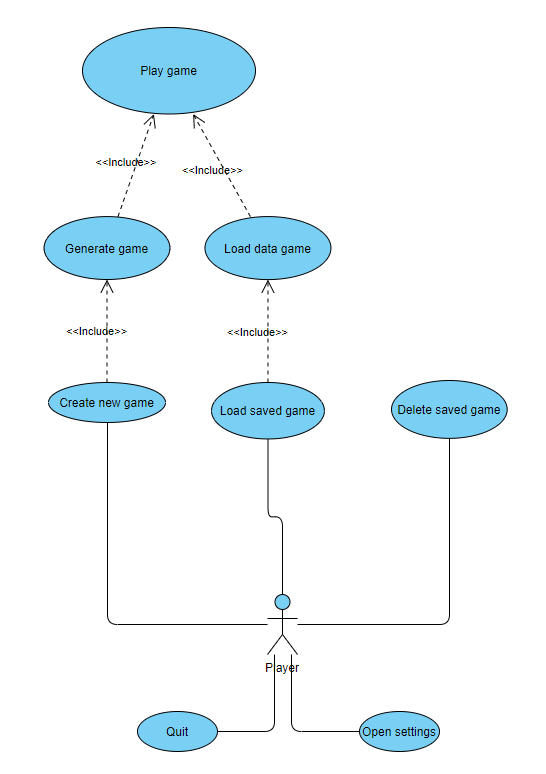
\includegraphics[width=0.5\linewidth]{images/useCaseMenu.png}
    \caption{Diagramme de use case du menu principal}
    \label{fig:useCaseMenu}
\end{figure}
Le joueur se trouve face à 5 possibilités représentées par 5 boutons : quitter le jeu, aller dans les paramètres, supprimer une partie sauvegardée, charger une partie sauvegardée ou créer une nouvelle partie.
\pagebreak

Le diagramme de use case du jeu se présente de la manière suivante :
\begin{figure}[H]
    \centering
    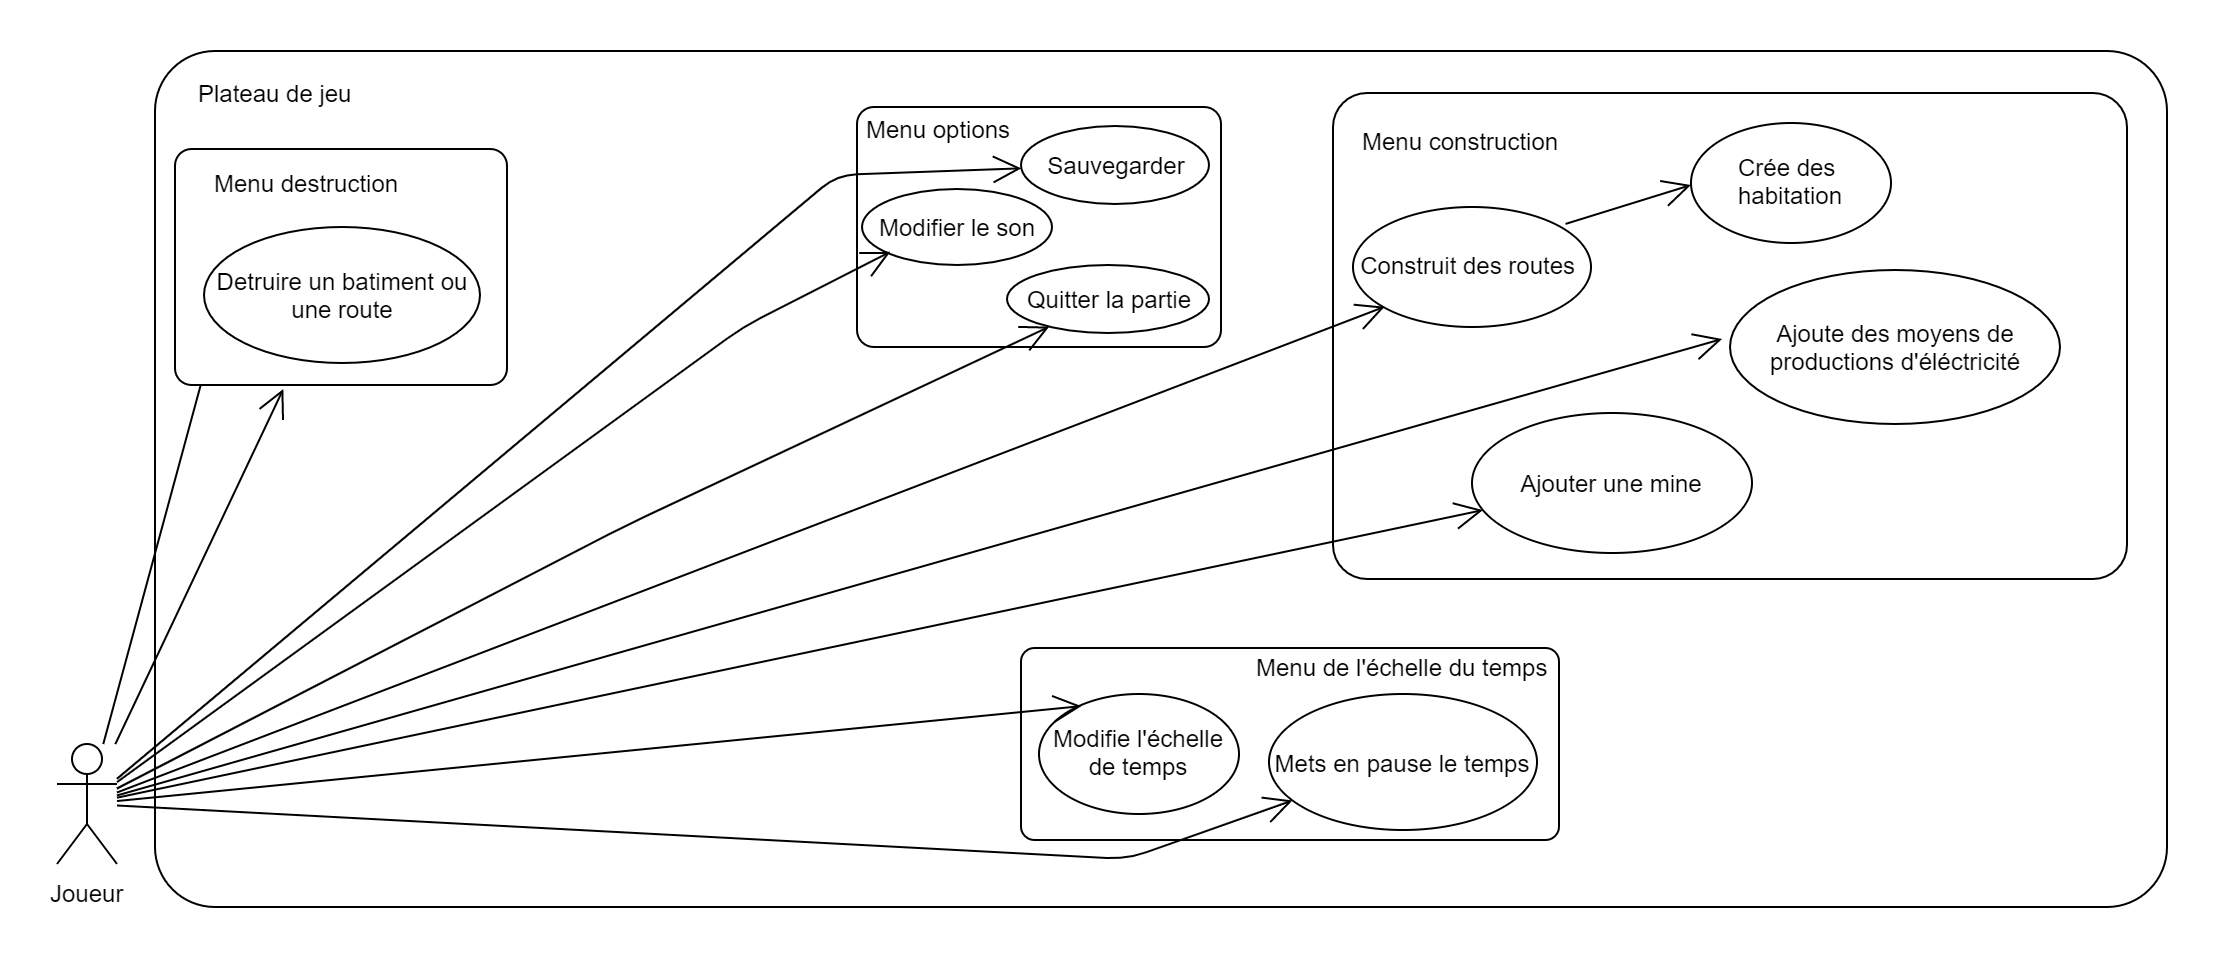
\includegraphics[width=1\linewidth]{images/Use-cases-1.png}
    \caption{Diagramme de use case en jeu}
    \label{fig:useCaseEnJeu}
\end{figure}
Afin de gérer sa ville le joueur et sa partie, le joueur peut faire 4 catégories d'actions séparées dans 4 menus.
Il peut soit :
\begin{itemize}
    \item[\textbullet] accélérer, ralentir ou mettre en pause le temps en jeu
    \item[\textbullet] détruire ce qu'il a construit
    \item[\textbullet]changer les paramètres du jeu si il ne l'a pas fait dans le menu principal
    \item[\textbullet]construire bâtiments, maisons et routes pour développer sa ville
\end{itemize}